\section{Résumé du cas clinique}

\subsection{Anamnèse}

\subsubsection{Contexte socio-culturel et clinique}
Patiente de $28$ ans, est d’origine Roumaine. Elle ne parle ni français ni néerlandais ni anglais ce qui impose la présence d’une interprète lors des différentes consultations. Elle est vierge et donc G0P0. Son cycle est spontané et dure $28$ jours. La date de ses dernières règles est le $02/06/2025$.

\subsubsection{Traitement actuel}
/

\subsubsection{Antécédents médicaux et chirurgicaux}
\begin{itemize}[label=\textbullet]
    \item \underline{$2018$} : Elle a présenté un kyste fonctionnel pour lequel la patiente était inquiète au point de devoir consulter. Cet antécédent n’est pas pertinent médicalement mais permet de mieux cerner la patiente.
    
    \item \underline{Août $2020$} : Une kystectomie splénique faite en Roumanie
    
    \item \underline{Septembre $2020$} : Une infection de plaie postopératoire reprise en Belgique (UCCLE) ainsi qu’un suivi à Bruges pour récidive de kystes spléniques.
\end{itemize}

\subsubsection{Affection actuelle}
\begin{itemize}[label=\textbullet]
    \item \underline{$6$ avril $2025$} : La patiente s’est présentée aux urgences pour dysménorrhée s’aggravant depuis 4 mois. Elle traite cette douleur cyclique par de l’Ibuprofène et Dafalgan sans pour autant pouvoir reprendre ses activités quotidiennes, il s’agit donc d’un grade III de dysménorrhée. Un scanner a été effectué et a révélé un kyste ovarien. L’hypothèse émise par l’urgentiste est un endométriome. A noter qu’au scanner, il est impossible de poser un    diagnostic quant à la nature du kyste.
    
    \item \underline{$5$ mai $2025$} : Lors d’une consultation gynécologique, l’examen clinique est sans particularité. L’échographie révèle un kyste ovarien uniloculaire en cycle spontané de $74\,x\,68\,x\,53$ mm à gauche compatible avec un endométriome. Une biologie qui reprend la réserve ovarienne ainsi que le CA $125$.
    
    \item \underline{$22$ mai $2025$} : La patiente se présente à un nouveau rendez-vous en gynécologie car elle souhaite une solution chirurgicale le plus vite possible. 
\end{itemize}

\subsection{Hypothèses diagnostiques}

\geometrieLarge
\begin{sidewaystable}
\centering
\caption{Les hypothèses diagnostiques}
\label{tab:hypothesesDiagnostiques}
\begin{tabular} {|>{\raggedright\arraybackslash}p{0.1\textwidth}|>{\raggedright\arraybackslash}p{0.2\textwidth}|>{\raggedright\arraybackslash}p{0.2\textwidth}|>{\raggedright\arraybackslash}p{0.2\textwidth}|>{\raggedright\arraybackslash}p{0.2\textwidth}|}
        \toprule
        Diagnostic & Définition & Symptômes & Signes cliniques & Remarques \\
        \midrule
        \hline
        Kyste hémorragique du corps jaune & Kyste fonctionnel, dépendant du cycle menstruel. & Dysménorrhée avec douleur unilatérale lors de la phase lutéale. & \vspace{-3mm} \begin{itemize}[label=\textbullet]
            \item Palpation abdominale : sensible ;
            \item Toucher vaginale : masse annexielle palpée, mobilisation utérine douloureuse.
        \end{itemize}
        & Rupture du kyste \rightarrow \hspace{5pt} défense abdominale, signe du cri du Douglas. \\
        \hline
        Endométriome & Endomètre ectopique au niveau ovarien. & Dysménorrhée, douleurs pelviennes chroniques, dyspareunie profonde, troubles de la fertilité. & \vspace{-3mm} \begin{itemize}[label=\textbullet]
            \item Palpation abdominale : sensible ;
            \item Toucher vaginale : masse annexielle palpable, mobilisation utérine douloureuse (adhérences suspectées), cul-de-sac du Douglas sensible.
        \end{itemize}
        & Les symptômes associés à d’autres systèmes sont observés (nycturie, dyschésie, trouble du transit, \ldots). Cependant, aucune explication scientifique ne parvient à établir un lien de causalité entre les symptômes et le kyste. \\
        \hline
        Kyste dermoïde & Tératome, tumeur bénigne d'origine embryonnaire, fréquente chez les femmes entre $16$ et $55$ ans. & Asymptomatique ou légère douleur pelvienne, métrorragie, dyspareunie et symptômes liés à une compression éventuelle. & \vspace{-3mm} \begin{itemize}[label=\textbullet]
            \item Palpation abdominale : normal ;
            \item Toucher vaginale : masse annexielle peut-être palpable. 
        \end{itemize}
        & Torsion ovarienne = urgence gynécologique \rightarrow \hspace{5pt} douleur abdominale aiguë et intense.  \\
        \hline
        Kyste para-ovarien & Kyste bénin avec pour origine le mésosaplinx. & Asymptomatique ou symptômes liés à une compression éventuelle. & \vspace{-3mm} \begin{itemize}[label=\textbullet]
            \item Palpation abdominale : normal ;
            \item Toucher vaginale : masse annexielle peut-être palpable. 
        \end{itemize}
        &  \\
        \hline
        \vspace{-3mm} Tumeur ovarienne & \vspace{-3mm} Cancer ovarien malin. Facteurs favorisants : G$0$P$0$, ménarche précoce, cycle menstruel spontané, \ldots & \vspace{-3mm} \parbox{0.2\textwidth}{Stade précoce : paucisymptomatique.\\
        Stade avancé : AEG, perte de poids, fatigue, \ldots} 
        & \vspace{-3mm} \begin{itemize}[label=\textbullet]
            \item Palpation abdominale : signes de carcinose (ventre de batracien, \ldots);
            \item toucher vaginale : masse annexielle palpable voire d'autres masses selon le stade d'extension.
        \end{itemize} & \vspace{-3mm} Ce diagnostic doit être exclu vu son pronostic dramatique. \\
        \hline
        \end{tabular}
\end{sidewaystable}
\geometrieWord

%\mbox{}
Les différentes hypothèses diagnostiques sont reprises dans le~\cref{tab:hypothesesDiagnostiques} à la~\cpageref{tab:hypothesesDiagnostiques}.

A noter que les examens cliniques de ces pathologies sont peu discriminants. Le diagnostic sera posé notamment grâce aux différents examens complémentaires dont l’imagerie.

\begin{figure}[H]
    \centering
    %\hspace*{-11mm}
    \begin{tcolorbox}[colframe=mdtRed, colback=white, boxrule=6pt, arc=30pt, halign=center, width=16cm]
    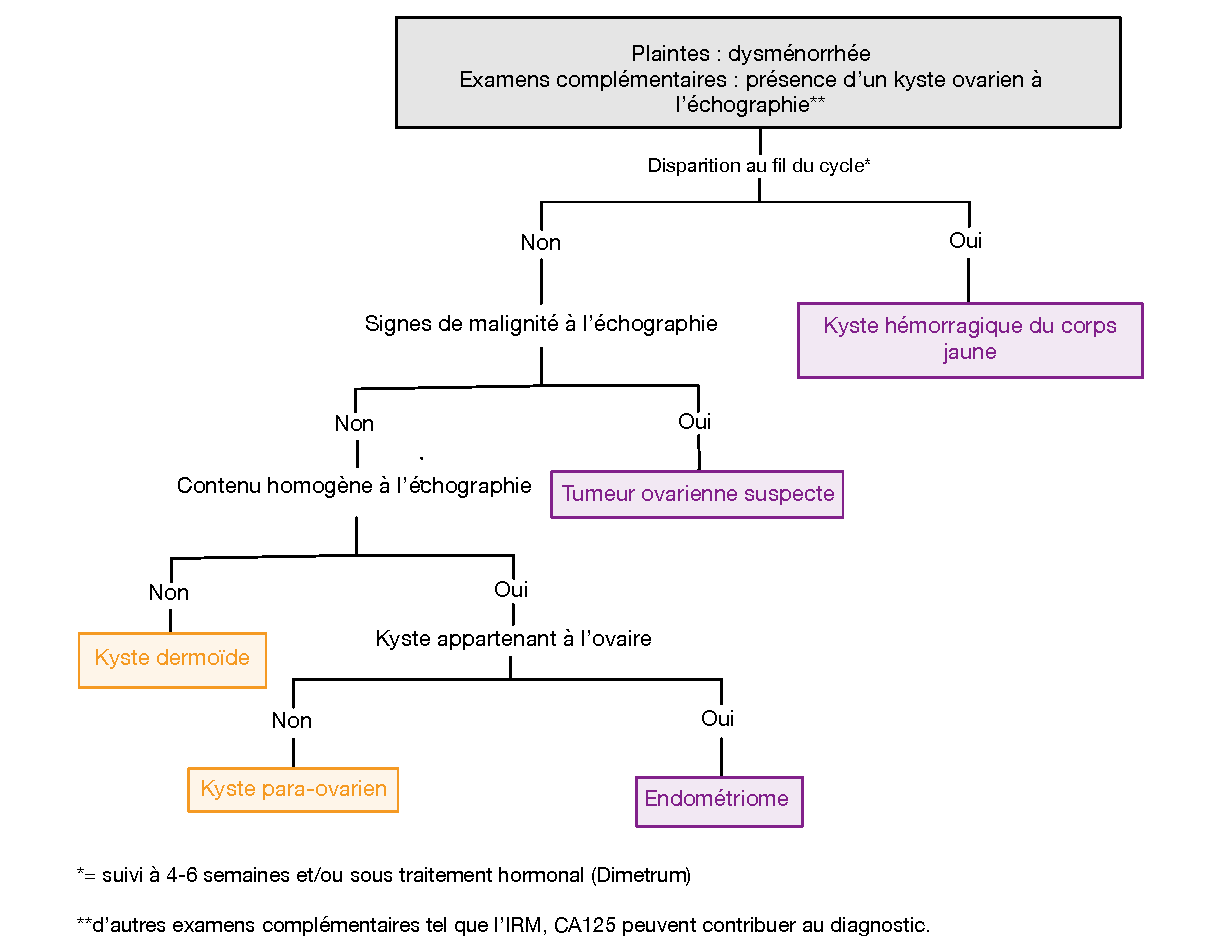
\includegraphics[width=14cm]{images/cas_diagnostique/schéma_DD.pdf}
    \end{tcolorbox}
    \caption{Arbre décisionnel des diagnostics différentiels d’un kyste ovarien chez une femme jeune en fonction de l’image échographique}
    \label{fig:ArbreDecisionMedical}
\end{figure}

\newpage

\subsection{Examen clinique} 
En gynécologie, l’examen clinique est souvent pauvre et il est nécessaire d’avoir une imagerie. Chez cette patiente, une palpation de l’abdomen a été réalisé. L’abdomen est souple, sans masse palpable. Toutefois, le toucher vaginal n’a pas été réalisé lors de la consultation car la patiente est vierge. Pourtant, un toucher vaginal pourrait donner des indications sur l’étendue de la pathologie. En effet, savoir qu’une mobilisation utérine est douloureuse ou la palpation d’autres masses éventuelles au niveau du ligament utéro-sacré, cul-de-sac de Douglas, \ldots{ } peut aider à orienter le diagnostic.

\subsection{Examens complémentaires}

\subsubsection{Biologie}
\begin{itemize}[label=\textbullet]
    \item \textbf{Justification :}\\
    une biologie a été réalisée dans le but d’évaluer le marqueur CA $125$, marqueur de l’irritation péritonéale. Son élévation est non spécifique mais présente lors d’endométriose profonde. La réserve ovarienne de la patiente est également estimé via l’AMH. Cette information aide à la prise de décision chirurgicale entre une kystectomie ou une annexectomie totale. L’hémoglobine et la coagulation sont aussi mesurées en cas de suspicion d’hémorragie intra-péritonéale et dans un contexte préopératoire proche.
    
    \item \textbf{Résultat :}%\\[0.3cm]
        \begin{table}[htbp]
\centering
\caption{Biologie - résultats}
\label{tab:examens_complementaires_resultat}
%\captionof{table}{Biologie - résultats}
\begin{tabular}{|p{0.2\textwidth}| p{0.2\textwidth}| p{0.2\textwidth}|}
    \toprule
    Nom & Quantité & Norme \\
    \midrule
    \hline
    AMH            & \SI{3.49}{\micro\gram\per\liter}         & \SIrange{1.18}{9.2}{\micro\gram\per\liter} \\
    \hline
    CA 125         & \SI{82}{\kilo\unit{U}\per\liter}         & <\SI{35}{\kilo\unit{U}\per\liter} \\
    \hline
    Hb             & \SI{13.2}{\gram\per\deci\liter}          & \SIrange{11.5}{16.5}{\gram\per\deci\liter} \\
    \hline
    PT (quick)     & \SI{92}{\percent}                        & >\SI{70}{\percent}, T25–35 \\
    \hline
    INR            & 1                                        & 1, T2.0–3.5 \\
    \hline
    aPTT           & \SI{29.8}{\second}                       & \SIrange{24.8}{34.4}{\second} \\
    \hline
    Fibrinogène    & \SI{262}{\milli\gram\per\deci\liter}     & \SIrange{200}{400}{\milli\gram\per\deci\liter} \\
    \hline
\end{tabular}
\end{table}
        %\\[1cm]
        
    \item \textbf{Impact :}\\
    L’interprétation de l’élévation de CA $125$ est complexe vu son aspécificité. Certes, lors d’endométriose profonde, le marqueur augmente mais c’est également le cas lors d’un cancer ovarien ou même lors d’un kyste fonctionnel provoquant une irritation péritonéale. Selon les autres examens, cette donnée pourra appuyer le diagnostic sans avoir un impact décisif sur celui-ci.
    
\end{itemize}

\subsubsection{Imagerie}

\begin{itemize}[label=\textbullet]
    \item \textbf{Justification :}\\
    Afin de poser le diagnostic, une échographie sera réalisée $5$ semaines après la première imagerie. Cet intervalle permet d’apprécier l’évolution du kyste. Pendant l’intervalle libre entre les deux imageries, la patiente prendra une pilule progestative, Dimetrum\textregistered dont sa principale indication thérapeutique est l’endométriose. Le Dime\-trum\textregistered\ est une pilule en continu, il induira une aménorrhée chez la patiente et inhibera l’ovulation ce qui exclura le kyste fonctionnel s’il persiste. Le Dimetrum\textregistered\ induit un environnement hypo-œstrogénique et hyperprogestogénique, ce qui entraîne une atrophie de l'endomètre eutopique et ectopique, diminuant ainsi les dysménorrhées. Un traitement hormonal joue donc un rôle diagnostic mais également thérapeutique.
    
    \item \textbf{Résultat :}\\
    Il est important de notifier que la patiente a affirmé avoir eu ses menstruations lors des $5$ semaines séparant les deux imageries. Ceci indique que la patiente n’a pas été compliante sur la prise du Dimetrum\textregistered.\, A l’échographie, le kyste ovarien gauche persiste. Il s’agit d’un kyste de $63\,x\,53\,x\,59$ mm uniloculaire avec des parois fines continues et finement échogènes ainsi qu’un Doppler négatif. En résumé, l’imagerie obtenue ne répond à aucun critère de malignité (taille > $6$ mm, paroi épaisse, présence de septa, présence d’ascite, présence d’hétérogénéité au sein de la masse annexielle)
    
    \item \textbf{Impact :}\\
    La persistance du kyste exclut définitivement le kyste hémorragique du corps jaune. Les caractéristiques du kyste sont bégnines. L’image et le contexte clinique sont fortement compatibles avec l’endométriome.
\end{itemize}

\subsubsection*{Justification de l'evidence-based diagnosis}
\addcontentsline{toc}{subsubsection}{Justification de l'evidence-based diagnosis}
La plupart des examens complémentaires réalisés sont cliniquement justifiés dans le cadre du diagnostic d’un endométriome. Cette approche est soutenue par de nombreux éléments retrouvés dans la littérature médicale. J’ai pu trouver une étude clinique, \textcite{nieva2024impact}, qui questionnait sur l’impact de l’évolution des guidelines du diagnostic de l’endométriose. Historiquement, la laparoscopie était le gold standard pour diagnostiquer \todoH{TestStyle}{green!30}{redondance et test de l'eapce commentaire à son maximum. Je t aime mon petit coeur de beurre. fjrea rgfre frf fr' frfa fraf frf 'hyh-' 'hgh fdnhdn hdngfd gd rehth erhg dngdb gehte h treht reh trehter h re hg erh ter ht hetr h  etgh getrh etyhtre hetrh htre htyh tek iut; u u, ut rzercz reb gtzrg gtrze rztre tgre regt tgt regtre tgrzeg treg trzg trgt rzg trzg trzg trzg tres grs gtr gtrze gtre zgtre zgt reg treg trz gtrz gt rzg trzg trz gtrz gt  grrg tre gtr eg treg tre gtr egt reg trzg trz gtre gt ergt reg t reg treg tre gt reg tre gt rz ze g rtv r trgt rgtregter tgre gtreg treg tregtreg gtrzg trz gtr g trzg trg tre tr eg  tzrgtr e tgre g trerteg tgr  rtg t rg trzg trz tg erg tre tgre  retgtr tr eg tre gtre t reg re trg e gt re gt re gt re}{l’endométriose}. Cette méthode présente pourtant des risques et les patientes y sont parfois réticentes. De plus, le lien de causalité entre l’étendue des lésions et la sévérité des symptômes reste incertain et complexe. D’autres inquiétudes apparaissent face à la laparoscopie qui pourrait retarder le diagnostic, voire sous-diagnostiquer les patientes. Donc, de nouvelles guidelines ont été établies par «European Society of Human Reproduction end Embryology» (ESHRE). Une approche multimodale a été adoptée, celle-ci prend en compte les symptômes des patientes ainsi que l’échographie transvaginale et l’IRM en complément de la laparoscopie pour diagnostiquer l’endométriose.  Les conclusions de cette étude clinique attestent que les recommandations, même les plus récentes, ont des limites. Elles ne permettent notamment pas de diagnostiquer l'ensemble des patientes en raison de l'hétérogénéité de la maladie et de ses symptômes. Il apparaît donc nécessaire d'élargir les critères et de replacer les symptômes au cœur de la démarche diagnostique. Cependant, l’évolution des guidelines a permis un diagnostic plus précoce par rapport à la laparoscopie seule mais cela n’est pas encore suffisant et de nombreux défis persistent.

Une autre méta-analyse, \textcite{kanti2024ultrasound}, a voulu comparer l’échographie transvaginale à l’IRM pour diagnostiquer l’endométriome. A nouveau, les différents essais cliniques qui confrontaient ces deux techniques étaient sujet à de nombreux biais. La comparaison de ces $2$ méthodes n’est donc pas évidente au niveau clinique vu le nombre d’études disponibles et leur qualité. Des critères peuvent, cependant, entrer en jeu tel que le coût, la disponibilité, \ldots{ } L’article tend à démontrer qu’il faut réaliser davantage d’études de comparaison mais que l’échographie et l’IRM sont deux imageries compétentes dans le diagnostic. Chacune des méthodes ayant leur avantages et inconvénients. Par exemple, l’échographie est plus accessible et moins onéreuse mais semble avoir un nombre de faux-positif plus élevé que l’IRM et donc moins spécifique. Dans notre cas, l’échographie était l’imagerie de choix vu son accessibilité et vu l’image détaillée et claire que nous avons obtenue. De plus, la laparoscopie thérapeutique permettra une seconde évaluation suffisante. L’IRM n’a donc pas sa place dans ce contexte.

Une étude multicentrique récente, \textcite{burghaus2024}\mbox{, }a évalué l’apport des biomarqueurs sanguins, notamment le CA $125$, dans le diagnostic de l’endométriose et de l’adénomyose. Les auteurs concluent qu’aucun biomarqueur seul ne permet actuellement de confirmer ou d’exclure avec certitude une endométriose. Toutefois, ils soulignent que le CA $125$ présente une bonne valeur diagnostique dans les formes sévères, en particulier en présence d’adhérences pelviennes ou d’un endométriome. En revanche, son utilité clinique diminue nettement dans les  autres formes. En cohérence avec ces limites, les recommandations du NICE et de l’ESHRE ne préconisent pas le dosage du CA $125$ comme outil diagnostique isolé, en raison de sa faible sensibilité et de sa variabilité interindividuelle. Dans notre cas, le dosage a été effectué, mais son interprétation reste délicate, et il n’apporte pas d’élément discriminant majeur dans la démarche diagnostique. Cet examen n’est pas inapproprié, mais il doit être interprété avec prudence et en complément d'autres éléments cliniques et radiologiques.

Pour aller plus loin dans la réflexion diagnostic, d’autres études comme \textcite{jiang2022diagnosis} questionnent l’utilité de l’intelligence artificielle dans le diagnostic de l’endométriose. Ceci est une preuve que de nouvelles pistes telles que l’intelligence artificielle doivent être explorées  car cette pathologie est encore trop souvent sous-diagnostiquée.

\subsection{Diagnostic}

\subsubsection{Diagnostic et sa présentation}
Le tableau clinique ainsi que les résultats obtenus lors des examens complémentaires sont grandement compatibles avec le diagnostic d’endométriome. L’endométriome est une forme particulière de l’endométriose. Cette maladie qui est la forme la plus fréquente et aussi appelée endométriome, est caractérisée par la présence de stroma et de glandes endométriales ectopiques notamment au niveau des ovaires. Ce kyste contient du sang couleur «chocolat» qui correspond à du vieux sang. L’endomètre ectopique est hormono-sensible et prolifère sous estrogènes pour se dégrader sous progestérone, tout comme l’utérus au cours du cycle. Le «vieux sang» correspond à la dégradation de l’endomètre qui ne peut être évacué et qui induirait des dysménorrhées.

\subsubsection{Ses répercussions}
Cette pathologie a un impact important sur le quotidien de la patiente. Les dysménorrhées ainsi que les autres symptômes empêchent la patiente d’assurer son quotidien. Son absentéisme professionnel a directement des conséquences négatives sur sa vie. Elle est sujet à la stigmatisation «des douleurs de règles». De plus, l’endométriome peut diminuer la fertilité voire rendre infertile la patiente.

\subsubsection{Traitement prescrit}
Deux alternatives de traitements ont été proposées à la patiente. D’une part un traitement de première ligne, un traitement hormonal, pour stabiliser la situation. Cependant, il s’agit d’un traitement symptomatique et il existe un risque d’expansion de la malade au niveau des trompes et des ovaires ce qui pourrait impacter davantage la fertilité. D’autre part, un traitement chirurgical par laparoscopie qui sera choisi par la patiente. Les indications de la chirurgie sont la dysménorrhée et le désir de grossesse. Vu la réserve ovarienne et l’âge de la patiente, une kystectomie est préférable à une annexectomie. La taille du kyste étant supérieure à 5mm, une kystectomie en deux temps peut être nécessaire avec une prise d’antagoniste GnRH entre les deux interventions dans le but d’atrophier les lésions endométriales. La laparoscopie permet également d’observer la cavité abdominale et de s’assurer que l’endométriose n’a pas envahi celle-ci.